\documentclass[table]{beamer}
%[]中可以使用handout、trancompress等参数
%usepackage[UTF8]{ctexcap}
%指定beamer的模式与主题
\mode<presentation>
{
  \usetheme{Madrid}
%\usetheme{Boadilla}
%\usecolortheme{default}
%\usecolortheme{orchid}
%\usecolortheme{whale}
%\usefonttheme{professionalfonts}
}

%\usetheme{Madrid}
%这里还可以选择别的主题:Bergen, Boadilla, Madrid, AnnArbor, CambridgeUS, Pittsburgh, Rochester, Warsaw, ...
%有导航栏的Antibes, JuanLesPins, Montpellier, ...
%有内容的Berkeley, PaloAlto, Goettingen, Marburg, Hannover, ...
%有最小导航栏的Berlin, Ilmenau, Dresden, Darmstadt, Frankfurt, Singapore, Szeged, ...
%有章和节表单的Copenhagen, Luebeck, Malmoe, Warsaw, ...

%\usecolortheme{default}
%设置内部颜色主题(这些主题一般改变block里的颜色);这个主题一般选择动物来命名
%这里还可以选择别的颜色主题,如默认的和有特别目的的颜色主题default,structure,sidebartab,全颜色主题albatross,beetle,crane,dove,fly,seagull,wolverine,beaver

%\usecolortheme{orchid}
%设置外部颜色主题(这些主题一般改变title里的颜色);这个主题一般选择植物来命名
%这里还可以选择别的颜色主题,如默认的和有特别目的的颜色主题lily,orchid,rose

%\usecolortheme{whale}
%设置字体主题;这个主题一般选择海洋动物来命名
%这里还可以选择别的颜色主题,如默认的和有特别目的的颜色主题whale,seahorse,dolphin

%\usefonttheme{professionalfonts}
%类似的还可以定义structurebold,structuresmallcapsserif,professionalfonts


% 控制 beamer 的风格,可以根据自己的爱好修改
%\usepackage{beamerthemesplit} %使用 split 风格
%\usepackage{beamerthemeshadow} %使用 shadow 风格
%\usepackage[width=2cm,dark,tab]{beamerthemesidebar}


% 设定英文字体
\usepackage{fontspec}
\setmainfont{Times New Roman}
\setsansfont{Arial}
\setmonofont{Courier New}

% 设定中文字体
\usepackage[BoldFont,SlantFont,CJKchecksingle,CJKnumber]{xeCJK}
%\setCJKmainfont[BoldFont={Adobe Heiti Std},ItalicFont={Adobe Kaiti Std}]{Adobe Song Std}
\setCJKmainfont[BoldFont={Heiti SC},ItalicFont={Kai}]{Hiragino Sans GB W3}
%\setCJKsansfont{Adobe Heiti Std}
%\setCJKmonofont{Adobe Fangsong Std}
\punctstyle{hangmobanjiao}

\defaultfontfeatures{Mapping=tex-text}
\usepackage{xunicode}
\usepackage{xltxtra}

\XeTeXlinebreaklocale "zh"
\XeTeXlinebreakskip = 0pt plus 1pt minus 0.1pt

\usepackage{setspace}
\usepackage{colortbl,xcolor}
\usepackage{hyperref}
%\hypersetup{xetex,bookmarksnumbered=true,bookmarksopen=true,pdfborder=1,breaklinks,colorlinks,linkcolor=blue,filecolor=black,urlcolor=cyan,citecolor=green}
\hypersetup{xetex,bookmarksnumbered=true,bookmarksopen=true,pdfborder=1,breaklinks,colorlinks,linkcolor=cyan,filecolor=black,urlcolor=blue,citecolor=green}

% 插入图片
\usepackage{graphicx}
% 指定存储图片的路径(当前目录下的figures文件夹)
\graphicspath{{figures/}}

% 可能用到的包
\usepackage{amsmath,amssymb}
\usepackage{multimedia}
\usepackage{multicol}
\usepackage{listings}

% 定义一些自选的模板,包括背景、图标、导航条和页脚等,修改要慎重
% 设置背景渐变由10%的红变成10%的结构颜色
%\beamertemplateshadingbackground{red!10}{structure!10}
%\beamertemplatesolidbackgroundcolor{white!90!blue}
% 使所有隐藏的文本完全透明、动态,而且动态的范围很小
\beamertemplatetransparentcovereddynamic
% 使itemize环境中变成小球,这是一种视觉效果
\beamertemplateballitem
% 为所有已编号的部分设置一个章节目录,并且编号显示成小球
\beamertemplatenumberedballsectiontoc
% 将每一页的要素的要素名设成加粗字体
\beamertemplateboldpartpage

% item逐步显示时,使已经出现的item、正在显示的item、将要出现的item呈现不同颜色
\def\hilite<#1>{
 \temporal<#1>{\color{gray}}{\color{blue}}
    {\color{blue!25}}
}

% 自定义彩色块状结构的颜色
\setbeamercolor{bgcolor}{fg=yellow,bg=cyan}

% 在表格、图片等得标题中显示编号
\setbeamertemplate{caption}[numbered]

% 打开PDF后直接全屏
\hypersetup{pdfpagemode={FullScreen}}


% 使用 \part,\section,\subsection 等命令组织文档结构
% 使用 \frame 命令制作幻灯片

\begin{document}

\logo{
\includegraphics[height=0.09\textwidth]{sysu.jpg}}
\title[PCA专题]{PCA学习}
\author[dalewzm]{王泽民}
\institute[SYSU]{School of Software\\ Sun-Yat Sen University}
\date{\today}

% 定义目录页
\AtBeginPart{
  \frame{
    \frametitle{\partpage}
    \begin{multicols}{2}
% 如果目录过长,可以打开这个选项分两栏显示
      \tableofcontents
% 使用这个命令自动生成目录
    \end{multicols}
  }  
}

% 在每个Section前都会加入的Frame
\AtBeginSection[]
{
  \begin{frame}<beamer>
    \frametitle{提纲}
	\setcounter{tocdepth}{2}
    \tableofcontents[currentsection,currentsubsection]
  \end{frame}
}
% 在每个Subsection前都会加入的Frame
\AtBeginSubsection[]
{
  \begin{frame}<beamer>
%\begin{frame}<handout:0>
% handout:0 表示只在手稿中出现
    \frametitle{提纲}
	\setcounter{tocdepth}{2}
    \tableofcontents[currentsection,currentsubsection]
% 显示在目录中加亮的当前章节
  \end{frame}
}

\begin{frame}
  \titlepage
\end{frame}

\begin{frame}[plain]
  \frametitle{提纲}
  \setcounter{tocdepth}{2}
  \tableofcontents
\end{frame}

\subsection{最大方差理论}
\begin{frame}
 在信号处理中认为信号具有较大的方差,噪声有较小的方差,信噪比就是信号与噪声的方差比,越大越好。如前面的图,样本在横轴上的投影方差较大,在纵轴上的投影方差较小,那么认为纵轴上的投影是由噪声引起的。

因此我们认为,最好的k维特征是将n维样本点转换为k维后,每一维上的样本方差都很大
\end{frame}

\subsection{最小错误理论}

\subsection{坐标轴相关度}


\section{降维与pca}
\begin{frame}
\frametitle{维度引发的问题}
\begin{itemize}
		\hilite <1> \item 大多数机器学习和数据挖掘算法的效率和复杂度和维度相关
	       \hilite <2> \item 维度信息的冗余,即某些维度之间有明显的关联
	       	\begin{example}
	   拿到一个汽车的样本,里面既有以“千米/每小时”度量的最大速度特征,也有“英里/小时”的最大速度特征
	\end{example}
	 \hilite <3> \item 一个样本,特征非常多,而样例特别少,这样用回归去直接拟合非常困难,容易过度拟合
	 \hilite <4> \item 在信号传输过程中,由于信道不是理想的,信道另一端收到的信号会有噪音扰动,那么怎么滤去这些噪音呢?
	\end{itemize}
\end{frame}
\begin{frame}
\frametitle{一句话介绍}
 \bf{PCA(Principal Component Analysis):}\\
 通过线性变换将原始数据变换为一组各维度\color{red}线性无关\color{black}的表示,可用于提取数据的\color{red}主要特征分量\color{black},常用于高维数据的\color{red}降维\color{black}
 \end{frame}
 



\section{PCA的过程与原理}
\begin{frame}
\frametitle{要搞清楚的问题}
  \begin{enumerate}
		  \item 什么是主成分?
		  \item 如何分析?
		  \item 怎么降维?
 \end{enumerate}
 \end{frame}
 

 \begin{frame}
 如果我们有M个N维向量,将其变换到R个N维向量表示的新空间中
 \it{p ,a}都是nx1\\
 \[\begin{pmatrix}
  p_1 \\
  p_2 \\
  \vdots \\
  p_R
\end{pmatrix}
\begin{pmatrix}
  a_1 & a_2 & \cdots & a_M
\end{pmatrix}
=
\begin{pmatrix}
  p_1a_1 &  p_1a_2 & \cdots & p_1a_M \\
  p_2a_1 &  p_2a_2 & \cdots &p_2a_M \\
  \vdots  &  \vdots  & \ddots & \vdots \\
  p_Ra_1 & p_Ra_2 & \cdots & p_Ra_M
\end{pmatrix}\]
 \end{frame}
 
 \begin{frame}
 先假定数据只有二维,即只有两个变量,它们由横坐标和纵坐标所代表;因此每个观测值(一个观测值就是图中的一个点)都有相应于这两个坐标轴的两个坐标值,
 我们数据有5条记录
 \[\begin{pmatrix}
  -1 & -1 & 0 & 2 & 0 \\
  -2 & 0 & 0 & 1 & 1
\end{pmatrix}\]
\begin{center}
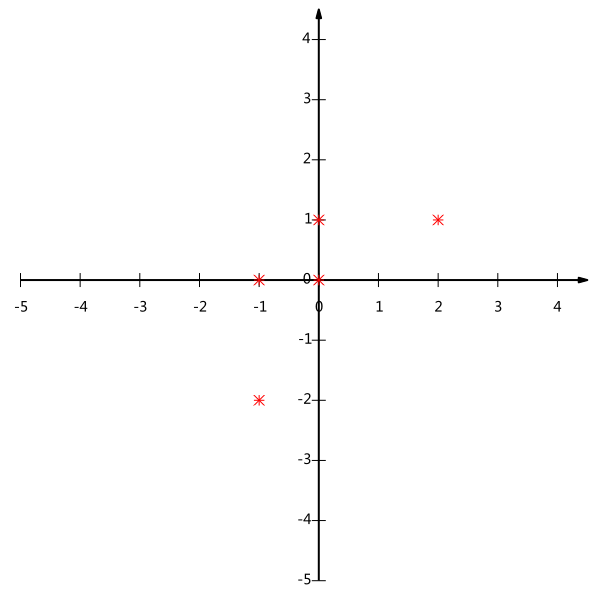
\includegraphics[height=4cm]{axis0.png}
\end{center}
 \end{frame}
 
 \begin{frame}
 \frametitle{如何降维}
 现在问题来了:如果我们必须使用一维来表示这些数据,又希望尽量保留原始的信息,你要如何选择?\\
一种直观的看法是:希望投影后的投影值尽可能分散。
  \end{frame}
  
  
  \begin{frame}
  而这种分散程度,可以用数学上的方差来表述
  $$Var(a)=\frac{1}{m}\sum_{i=1}^m{(a_i-\mu)^2}$$
  在实际应用时,我们可以先将每个字段均值化为0(将每个数据预先减去均值)
  $$Var(a)=\frac{1}{m}\sum_{i=1}^m{a_i^2}$$
  \end{frame}
  
  
  
  \begin{frame}
  \frametitle{协方差}
  数学上可以用两个字段的协方差表示其相关性
  $$Cov(X, Y) = E[(X - \mu_X)(Y - \mu_Y)]$$
  由于已经让每个字段均值为0,\\
  $$Cov(a,b)=\frac{1}{m}\sum_{i=1}^m{a_ib_i}$$
  在字段均值为0的情况下,两个字段的协方差简洁的表示为其内积除以元素数m。

当协方差为0时,表示两个字段不相关
  \end{frame}
  
  \begin{frame}
  \frametitle{协方差矩阵}
  假设我们只有a和b两个字段,那么我们将它们按行组成矩阵X
  \[X=\begin{pmatrix}
  a_1 & a_2  &\cdots & a_m \\
  b_1 & b_2  &\cdots & b_m
\end{pmatrix}\]
然后我们用X乘以X的转置,并乘上系数1/m\\
\[\frac{1}{m}XX^\mathsf{T}=\begin{pmatrix}
  \frac{1}{m}\sum_{i=1}^m{a_i^2}   & \frac{1}{m}\sum_{i=1}^m{a_ib_i} \\
  \frac{1}{m}\sum_{i=1}^m{a_ib_i} & \frac{1}{m}\sum_{i=1}^m{b_i^2}
\end{pmatrix}\]
这个矩阵对角线上的两个元素分别是两个字段的方差,而其它元素是a和b的协方差。两者被统一到了一个矩阵的。

这个结论很容易被推广到一般情况:
设\(C=\frac{1}{m}XX^\mathsf{T}\),则C是一个对称矩阵,其对角线分别个各个字段的方差,而第i行j列元素表示i和j两个字段的协方差
  \end{frame}
  
  \begin{frame}
  但我们希望的是,投影到该维度上方差最大,维度间无关,即协方差为0,那么这样的矩阵就是对角矩阵
  即除对角线外的其它元素化为0,并且在对角线上将元素按大小从上到下排列,这样我们就达到了目的
  \end{frame}
  
  \begin{frame}
  设原始数据矩阵X对应的协方差矩阵为C\\而P是一组基按行组成的矩阵\\
  设Y=PX,则Y为X对P做基变换后的数据。Y的协方差矩阵为D.\\我们推导一下D与C的关系
  \[\begin{array}{l l l}
  D &= &\frac{1}{m}YY^\mathsf{T} \\
    &= &\frac{1}{m}(PX)(PX)^\mathsf{T} \\
    & = & \frac{1}{m}PXX^\mathsf{T}P^\mathsf{T} \\
    &= &P(\frac{1}{m}XX^\mathsf{T})P^\mathsf{T} \\
    & = & PCP^\mathsf{T}
\end{array}\]
  \end{frame}
  
  
  \begin{frame}
  协方差矩阵C是一个是对称矩阵,在线性代数上,实对称矩阵有一系列非常好的性质:\\
   \begin{enumerate}
\item 实对称矩阵不同特征值对应的特征向量必然正交。
\item 设特征向量λ重数为r,则必然存在r个线性无关的特征向量对应于λ,因此可以将这r个特征向量单位正交化。
\end{enumerate}
  \end{frame}
  
  \begin{frame}
  由上面两条可知,一个n行n列的实对称矩阵一定可以找到n个单位正交特征向量,设这n个特征向量为e1,e2,....,$e_n$,我们将其按列组成矩阵:
  \[E=\begin{pmatrix}
  e_1 &  e_2 & \cdots &  e_n
\end{pmatrix}\]
则对协方差矩阵C有如下结论:
\[E^\mathsf{T}CE=\Lambda=\begin{pmatrix}
  \lambda_1 &           &     &\\
              &  \lambda_2 &      & \\
              &            & \ddots &\\
              &           &      &\lambda_n
\end{pmatrix}\]
其中\(\Lambda\)为对角矩阵,其对角元素为各特征向量对应的特征值(可能有重复)
  \end{frame}
  
 
  
  \begin{frame}
  总结一下PCA的算法步骤:
  设有m条n维数据。
  \begin{columns}
  \column{4cm}
  \begin{block}{步骤1}
将原始数据按列组成n行m列矩阵X
\end{block}
\column{4cm}
\begin{example}
这里以上文提到的数据
\[\begin{pmatrix}
  -1 & -1 & 0 & 2 & 0 \\
  -2 & 0  & 0 & 1 & 1
\end{pmatrix}\]
\end{example}
\end{columns}
  \end{frame}
  
  
  \begin{frame}
  \begin{columns}
  \column{4cm}
  \begin{block}{步骤2}
  将X的每一行(代表一个属性字段)进行零均值化,即减去这一行的均值
  \end{block}
  \column{4cm}
  \begin{example}
   因为这个矩阵的每行已经是零均值,这里我们直接求协方差矩阵:
   \end{example}
  \end{columns}
  \end{frame}
  
  
   \begin{frame}
  \begin{columns}
  \column{3cm}
  \begin{block}{步骤3}
求出协方差矩阵\(C=\frac{1}{m}XX^\mathsf{T}\)
\end{block}
  \column{6cm}
  \begin{example}
   因为这个矩阵的每行已经是零均值,这里我们直接求协方差矩阵:
   
   \[C=\frac{1}{5}\begin{pmatrix}
  -1 & -1 & 0 & 2 & 0 \\
  -2 & 0 & 0 & 1 & 1
\end{pmatrix}\begin{pmatrix}
  -1 & -2 \\
  -1 & 0  \\
  0  & 0  \\
  2  & 1  \\
  0  &1
\end{pmatrix}\] \\ \[= \begin{pmatrix}
  \frac{6}{5} & \frac{4}{5} \\
  \frac{4}{5} &\frac{6}{5}
\end{pmatrix}\]
\end{example}
  \end{columns}
  \end{frame}
  
   \begin{frame}
  \begin{columns}
  \column{4cm}
  \begin{block}{步骤4}
  求出协方差矩阵的特征值及对应的特征向量
  \end{block}
  \column{4cm}
  \begin{example}
   求解后特征值为:
   \[\lambda_1=2,\lambda_2=2/5\]
   其对应的特征向量分别是:
   \[c_1\begin{pmatrix}
  1 \\
  1
\end{pmatrix},c_2\begin{pmatrix}
  -1 \\
  1
\end{pmatrix}\]
\end{example}
  \end{columns}
  \end{frame}
  
  \begin{frame}
  \begin{columns}
  \column{4cm}
  \begin{block}{步骤5}
将特征向量按对应特征值大小从上到下按行排列成矩阵,取前k行组成矩阵P
\end{block}
  \column{4cm}
  \begin{example}
降维,取一行\\
\[P=\begin{pmatrix}
  1/\sqrt{2}   \\
  1/\sqrt{2} 
  \end{pmatrix}\]
  \end{example}
  \end{columns}
  \end{frame}
  
  \begin{frame}
  \begin{columns}
  \column{2cm}
  \begin{block}{步骤6}
Y=PX即为降维到k维后的数据
\end{block}
  \column{6cm}
  \begin{example}
  \[Y=\begin{pmatrix}
  1/\sqrt{2} & 1/\sqrt{2}
\end{pmatrix}\begin{pmatrix}
  -1 & -1 & 0 & 2 & 0 \\
  -2 & 0 & 0 & 1 & 1
\end{pmatrix}= \] \\ \[ \begin{pmatrix}
  -3/\sqrt{2} &-1/\sqrt{2} & 0 & 3/ \sqrt{2} & -1/\sqrt{2}
\end{pmatrix}\]
\end{example}
  \end{columns}
  \end{frame}
  
 \subsection{重新梳理}
 \begin{frame}
以二维为例:数据形成一个椭圆形状的点阵
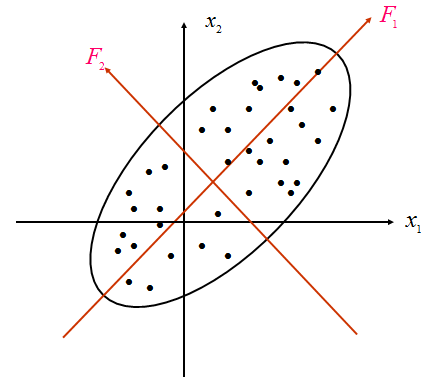
\includegraphics[height = 5cm]{pca1.png}
 \end{frame}
 
\begin{frame}
椭圆有一个长轴和一个短轴。在短轴方向上,数据变化很少;\\
在极端的情况,短轴如果退化成一点,那只有在长轴的方向才能够解释这些点的变化了;\\
这样,由二维到一维的降维就自然完成了。
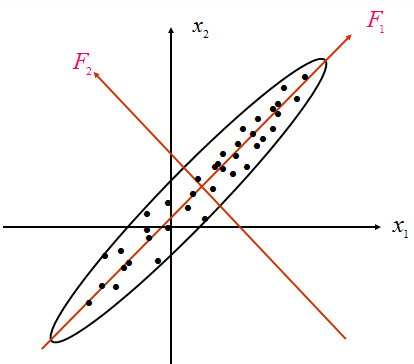
\includegraphics[height = 5cm]{pca2.png}
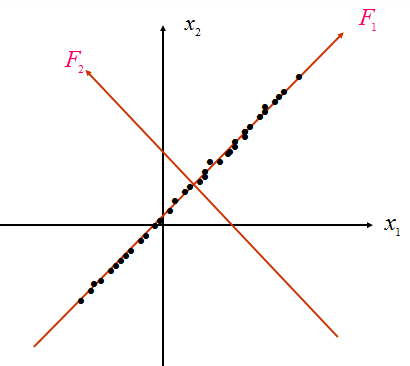
\includegraphics[height = 5cm]{pca3.png}
\end{frame}

\begin{frame}
首先把高维椭球的主轴找出来,再用代表大多数数据信息的最长的几个轴作为新变量;\\
和二维情况类似,高维椭球的主轴也是互相垂直的。这些互相正交的新变量是原先变量的线性组合,叫做主成分\\
数据的主要成分(即特征向量)与它们的权值(即特征值)
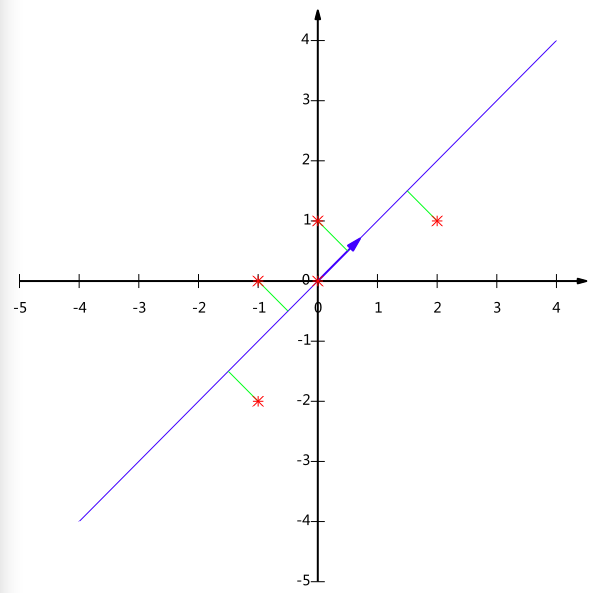
\includegraphics[height=5cm]{axis_ans.png}
\end{frame}


\section{PCA的应用与实现}
\begin{frame}
\frametitle{实战pca}
人脸数据集:
\href{www.cbcl.mit.edu/software-datasets/FaceData2.html}{mit CBCL人脸数据库}\\
人脸保存为灰度图像,为pgm格式,19*19\\
代码为matlab
\end{frame}




\begin{frame}[fragile]
\begin{lstlisting}[language=Matlab]
numOfPic = 10;
trainSet = zeros( numOfPic, 19*19 ); 
for i = 1 : numOfPic
     str=sprintf('face/face%05d.pgm',i);
     img = imread( str );   
     img = double(img);
     trainSet(i,:) = img(:);
end
\end{lstlisting}
图像分辨率:19*19\\
文件名:faceXXXXX.pgm
trainSet维数:10x361
\end{frame}


\begin{frame}[fragile]
\begin{lstlisting}[language=Matlab]
meanValue = mean( trainSet );

trainSet_norm = bsxfun(@minus,trainSet, meanValue);
sigma = std(trainSet_norm); %每一列的标准差
trainSet_norm = bsxfun(@rdivide, 
                trainSet_norm, sigma);
imwrite(uint8(
              reshape(meanValue,19,19)),'mean.bmp');
\end{lstlisting}
数据标准化
\end{frame}

\begin{frame}
\frametitle{数据标准化}
\begin{block}{标准化}
对原始数据进行缩放处理,限制在一定的范围内。一般指正态化,即均值为0,方差为1。即使数据不符合正态分布,也可以采用这种方式方法,标准化后的数据有正有负
\end{block}
目的是为了进行数据无量纲化,解决数据的可比性\\
一般灰度图像无需此处理
\end{frame}


\begin{frame}[fragile]
\frametitle{协方差矩阵与特征值}
\begin{lstlisting}[language=Matlab]
X = trainSet_norm;
[m, n] = size(X);
Cov = 1/m*X'*X;
[U ,S, V] =svd(Cov);
\end{lstlisting}
奇异值与特征值\\
对称矩阵特征值与奇异值差正负号,特征向量和奇异向量张成空间一样。从谱分解来看,对称矩阵可以酉对角化,$A=Q*B*Q^t$,B对角线特征值,只要将负号加到Q的列上,使B对角线大于0,得到的就是奇异值分解\\
svd得到的奇异值是按降序排列的
\end{frame}
\begin{frame}
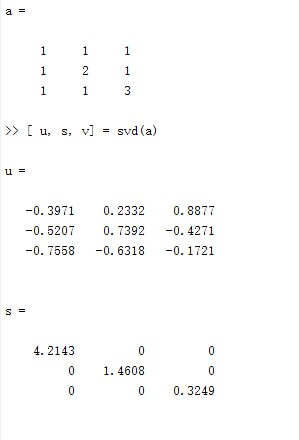
\includegraphics[width=5cm]{pca10.jpg}
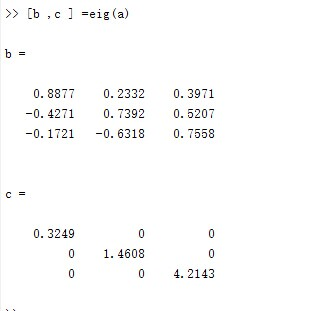
\includegraphics[height=5cm]{pca11.jpg}
\end{frame}

\begin{frame}[fragile]
\frametitle{降到多少维}
\begin{lstlisting}[language=Matlab]
eigValue = diag(S);
AllSum = sum(eigValue);
cur_Sum = 0;
p =0;
while( cur_Sum/ AllSum < 0.9)
	p = p + 1;
        cur_Sum = sum(eigValue(1:p));
end;
P = U(:, 1:p);
\end{lstlisting}
选择主轴成分比重0.9以上,比重是可以自己定的,一般大于0.85,丢失的信息才不多
\end{frame}


\subsection{princomp介绍}
\begin{frame}
\frametitle{matlab自带主成分分析函数}
[COEFF,SCORE,latent,tsquare] = princomp(X)\\
1.输入参数 X 是一个 n 行 p 列的矩阵。每行代表一个样本观察数据,每列则代表一个属性,或特征\\
2COEFF 就是所需要的特征向量组成的矩阵,是一个 p 行 p 列的矩阵,
每,经常也称为(协方差矩阵的)特征向量。
并且是按照对应特征值降序排列的。所以,如果只需要前 k 个主成分向量,
可通过:COEFF(:,1:k) 来获得。\\
3.SCORE 表示原数据在各主成分向量上的投影。但注意:是原数据经过中心化后在主成分向量上的投影
SCORE = x0*COEFF 求得。其中 x0 是中心平移(减去均值)后的X\\
4、latent 是一个列向量,表示特征值,并且按降序排列。
\end{frame}

\begin{frame}
\begin{center}
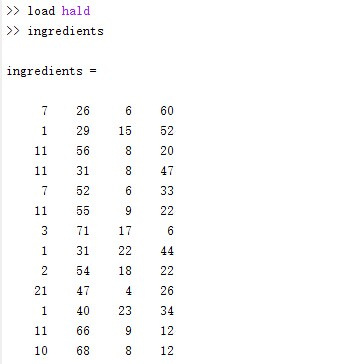
\includegraphics[height=8cm]{in0.jpg}
\end{center}
\end{frame}


\begin{frame}
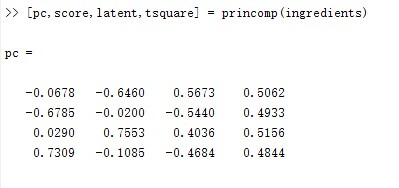
\includegraphics[width=5cm]{in1.jpg}
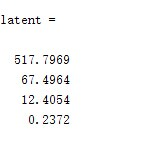
\includegraphics[width=3cm]{in2.jpg}
\end{frame}

\begin{frame}
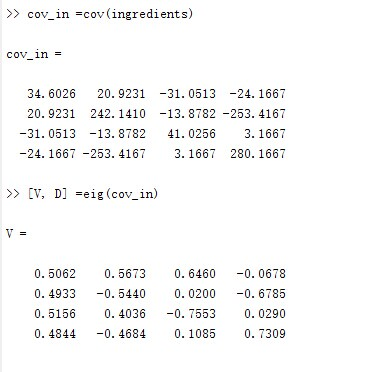
\includegraphics[width=5cm]{in3.jpg}
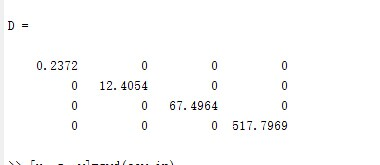
\includegraphics[width=5cm]{in4.jpg}
\end{frame}


\begin{frame}
 meanValue = mean(ingredients)\\

meanValue =\\
\begin{table}
\begin{tabular}{|c|c|c|c|}
\hline
  \rowcolor{blue!50}  7.4615 &  48.1538 &  11.7692  & 30.0000\\
  \hline
  \end{tabular}
  \end{table}

 a = bsxfun(\@minus,ingredients,meanValue);

1/12*a'*a\\
ans =
\begin{table}
\rowcolors[]{1}{blue!20}{blue!10}
\begin{tabular}{|c|c|c|c|}
\hline
   34.6026 &  20.9231 & -31.0513&  -24.1667\\
   20.9231&  242.1410  &-13.8782& -253.4167\\
  -31.0513  &-13.8782  & 41.0256 &   3.1667\\
  -24.1667 &-253.4167 &   3.1667 & 280.1667\\
    \hline
  \end{tabular}
  \end{table}
 \end{frame} 

\subsection{在图形学的其它一些应用}
\begin{frame}
\frametitle{降维找数据的分布特征}
分析网格数据(如对人物的网格进行分析从而发现其骨架拓扑)时,有时会得到一堆散乱分布在关节附近的顶点数据,利用主元分析对这些散乱的顶点进行降维,如从3维降到2维,则可以发现这些顶点数据的分布特征。\\

\end{frame}

  
\begin{frame}
\frametitle{三角形网格的有向包围盒(OBB)}
OBB是一种对模型进行视锥裁剪与碰撞检测的有效方式,然而通常网格模型表示在一个与世界坐标系平行的框架中,可以利用主元分析求得模型所在的各个自然轴,如一个斜放着的圆柱其第一个自然轴是有圆柱底面中心指向圆柱顶面中心的方向。求得各个自然轴后,通过各顶点坐标与单位自然轴的点积,即可获得各顶点在自然轴上的分布范围,进而得到OBB。
\end{frame}
\begin{frame}
\frametitle{人物动画特征提取}
例如数据捕捉采集到的人体步行动画通常由不同时刻各个关节(约40~60个)的角度来表示,当数据量很大时,对数据的存储与处理都是一件耗费资源的事情。而普通的步行动作中,当一个人左臂向前摆动时右臂总向后摆动,这就是说这些数据有耦合,从而可以利用主元分析进行特征提取与压缩。由此也可以想象得到主元分析另一个强大的地方:对于一些高维度的数据,很难用三维图形的方式去展现,因此很难观察出其分布特征,而主元分析计算则可以发现这些特征。
\end{frame}





\section{PCA的进一步讨论}
\begin{frame}
根据上面对PCA的数学原理的解释,我们可以了解到一些PCA的能力和限制。PCA本质上是将方差最大的方向作为主要特征,并且在各个正交方向上将数据“离相关”,也就是让它们在不同正交方向上没有相关性。\\
因此,PCA也存在一些限制,
\begin{itemize}
		\hilite <1> \item 它可以很好的解除线性相关,但是对于高阶相关性就没有办法了
		 \begin{block}{解决办法}
		 对于存在高阶相关性的数据,可以考虑Kernel PCA,通过Kernel函数将非线性相关转为线性相关,关于这点就不展开讨论了
		 \end{block}
	       \hilite <2> \item PCA假设数据各主特征是分布在正交方向上,如果在非正交方向上存在几个方差较大的方向,PCA的效果就大打折扣了
	      
	
	\end{itemize}


\end{frame}


\begin{frame}
本文档使用或参考了以下来源内容:\\
\href{http://www.melory.me}{melory博客主成份分析}\\
\href{http://blog.codinglabs.org/articles/pca-tutorial.html}{pca-tutorial}\\
\href{https://ccjou.wordpress.com/2013/04/15/主成分分析}{线代启示录-主成分分析(网站需要翻墙)}
\end{frame}



\end{document}
